\documentclass{standalone}
\usepackage{tikz}
\usetikzlibrary{positioning, shapes.geometric, calc}

\begin{document}

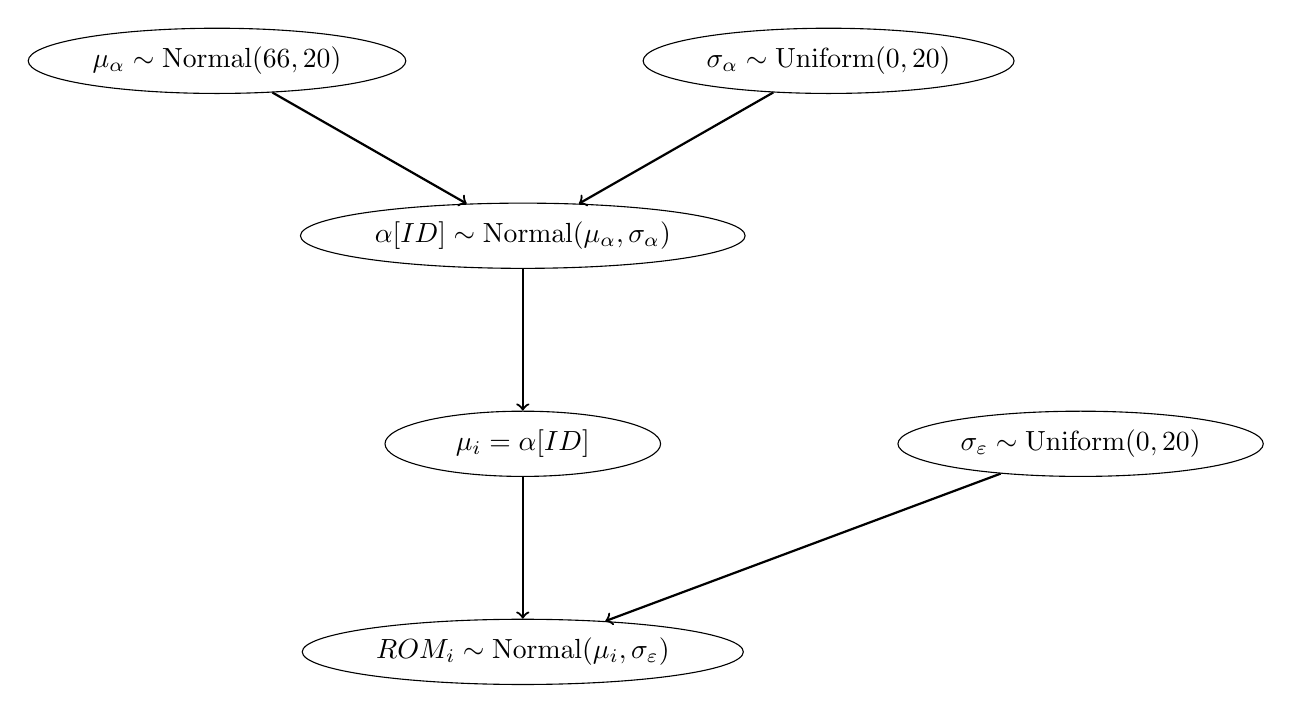
\begin{tikzpicture}[
    node distance=1.8cm and 3cm,
    every node/.style={draw, ellipse, align=center, minimum width=3.5cm, font=\normalsize}
]

% Nodes
\node (mualpha) {\(\mu_\alpha \sim \mathrm{Normal}(66, 20)\)};
\node (sigmaalpha) [right=of mualpha] {\(\sigma_\alpha \sim \mathrm{Uniform}(0, 20)\)};
\node (alphaID) [below=of $(mualpha)!0.5!(sigmaalpha)$] {\(\alpha[ID] \sim \mathrm{Normal}(\mu_\alpha, \sigma_\alpha)\)};
\node (mui) [below=of alphaID] {\(\mu_i = \alpha[ID]\)};
\node (sigmaepsilon) [right=of mui] {\(\sigma_\varepsilon \sim \mathrm{Uniform}(0, 20)\)};
\node (ROMi) [below=of mui] {\(ROM_i \sim \mathrm{Normal}(\mu_i, \sigma_\varepsilon)\)};

% Arrows
\draw[->, thick] (mualpha) -- (alphaID);
\draw[->, thick] (sigmaalpha) -- (alphaID);
\draw[->, thick] (alphaID) -- (mui);
\draw[->, thick] (mui) -- (ROMi);
\draw[->, thick] (sigmaepsilon) -- (ROMi);

\end{tikzpicture}

\end{document}